% Chapter Template

\chapter{Emulation REPTAR} % Main chapter title

\label{Chapitre 3} % Change X to a consecutive number; for referencing this chapter elsewhere, use \ref{ChapterX}

\lhead{ \emph{Emulation REPTAR}} % Change X to a consecutive number; this is for the header on each page - perhaps a shortened title

%----------------------------------------------------------------------------------------
%	SECTION 1
%----------------------------------------------------------------------------------------
Ce chapitre s'intéresse principalement aux différents périphériques hardware émulés de la REPTAR, à l'aide du framework QEmu.

\section{Etapes}
Voici les quelques étapes importantes développées au cours de ce laboratoire. 

\subsection{Etape 2}
Cette étape nous a permis d'émuler la FPGA (y compris le bus reliant la Spartan6 et l'OMAP).\\


Voici quelques parties de code importants pour émuler la FPGA, ainsi que les différents registres qui la composent. Ici, le bus de communication est abstrait. On n'émule pas les différents signaux de communication (pas de bus AMBA ou AXI).\\

Pour commencer, voici la déclaration de notre périphérique FPGA, avec les deux fonctions d'initialisation correspondantes : 
\begin{lstlisting}[language=C,caption=Spartan 6 device declaration]

static const TypeInfo reptar_sp6_info = { 
	.name = "reptar_sp6", 
	.parent = TYPE_SYS_BUS_DEVICE, 
	.instance_size = sizeof(sp6_state_t),
	.instance_init = sp6_init, 
	.class_init = sp6_class_init, 
	};

static void sp6_class_init(ObjectClass *klass, void *data) {
	SysBusDeviceClass *k = SYS_BUS_DEVICE_CLASS(klass);
	k->init = sp6_initfn;
}

static void sp6_init(Object *obj) {
	// do nothing...
}	
\end{lstlisting}

On voit que l'on a une fonction "sp6\_initfn". Elle sera appelée à l'initialisation de la classe de périphérique de ce type.\\
\pagebreak
Voici le code de cette fonction :  
\begin{lstlisting}[language=C,caption=Device initialization]

static int sp6_initfn(SysBusDevice *sbd) {
	DeviceState *dev = DEVICE(sbd);
	sp6_state_t *s = OBJECT_CHECK(sp6_state_t, dev, "reptar_sp6");

	memory_region_init_io(&s->iomem, OBJECT(s), &sp6_ops, s, "reptar_sp6",
			0x1000);
	sysbus_init_mmio(sbd, &s->iomem);

	memset(&s->regs, 0, sizeof(s->regs));

	sysbus_init_irq(sbd, &s->irq);

	sp6_emul_init();
	reptar_sp6_leds_init(s);
	reptar_sp6_btns_init(s);
	reptar_sp6_irq_init(s);
	reptar_sp6_7segs_init(s);

	DBG("sp6_initfn : initialization de la FPGA...\n");

	return 0;
}
\end{lstlisting}

On voit que cette fonction initialise tout les périphériques de la FPGA (LEDs, boutons, etc.) en plus de réserver sa mémoire. Les interruptions sont aussi initialisées dans cette section de code.\\

Voyons maintenant les fonctions d'accès en lecture et en écriture sur le bus de la FPGA :
\begin{lstlisting}[language=C,caption=FPGA bus IO access]

static uint64_t sp6_read(void *opaque, hwaddr addr, unsigned size) {
	uint64_t ret_value = 0;

	// Récupération de la structure d'état
	sp6_state_t *sp6_dev_struct_ptr = (sp6_state_t*) opaque;

	switch ((uint8_t) addr) {
	case SP6_IRQ_STATUS:
		break;
	case SP6_PUSH_BUT:
		ret_value = reptar_sp6_btns_read();
		break;
	case SP6_IRQ_CTL:
		ret_value = reptar_sp6_irq_read();
		break;
	case SP6_7SEG1:
		reptar_sp6_7segs_read(SP6_7SEG1);
		break;
	case SP6_7SEG2:
		ret_value = reptar_sp6_7segs_read(SP6_7SEG2);
		break;
	case SP6_7SEG3:
		ret_value = reptar_sp6_7segs_read(SP6_7SEG3);
		break;
	case SP6_LCD_CONTROL:
	case SP6_LCD_STATUS:
		DBG("sp6_read %08x bytes @%08x\n", (uint32_t )size, (uint32_t )addr);
		break;
	case SP6_LED:
		ret_value = reptar_sp6_leds_read();
		break;
	default:
		DBG("Error, no valid register address!\n");
		break;
	}

	return (uint64_t) ret_value;
}

static void sp6_write(void *opaque, hwaddr addr, uint64_t value, unsigned size) {
	// Récupération de la structure d'état
	sp6_state_t *sp6_dev_struct_ptr = (sp6_state_t*) opaque;

	switch ((uint8_t) addr) {
	case SP6_IRQ_STATUS:
	case SP6_PUSH_BUT:
		break;
	case SP6_IRQ_CTL:
		reptar_sp6_irq_write((uint8_t) value);
		break;
	case SP6_7SEG1:
		reptar_sp6_7segs_write((uint8_t) value, SP6_7SEG1);
		break;
	case SP6_7SEG2:
		reptar_sp6_7segs_write((uint8_t) value, SP6_7SEG2);
		break;
	case SP6_7SEG3:
		reptar_sp6_7segs_write((uint8_t) value, SP6_7SEG3);
		break;
	case SP6_LCD_CONTROL:
	case SP6_LCD_STATUS:
		DBG("sp6_write %08x bytes, value = %08x, @%08x\n", (uint32_t )size,
				(uint32_t )value, (uint32_t )addr);
		break;
	case SP6_LED:
		reptar_sp6_leds_write((uint8_t) value);
		break;
	default:
		DBG("Error, no valid register address!\n");
		break;
	}
}
\end{lstlisting}

\pagebreak
Voici ci-dessous la déclaration de la structure "opaque" qui sera utilisée dans nos différents modules d'émulation : 
\begin{lstlisting}[language=C,caption=Opaque struct definition]
typedef struct
{
    SysBusDevice busdev;
    MemoryRegion iomem;
    uint16_t regs[512];		/* 1KB (512 * 16bits registers) register map */
    qemu_irq irq;
} sp6_state_t;
\end{lstlisting}

Nous avons utilisé des registres de 16bits, comme donné dans le plan mémoire de la FPGA.
Le décodage d'adresses est fait dans cette portion de code. On appelle les fonctions correspondantes aux périphériques concernés, soit en lecture, soit en écriture.\\

\textit{\textbf{Remarque} : Une chose étrange est le type "uint64\_t", alors que notre architecture est de 32bits (bien que actuellement les processeurs ARM arrivent en 64 bits). Il faudra donc faire attention à l'alignement utilisé!}

Tests effectués : pour tester si ce code fonctionne nous avons fait une lecture à l'adresse du LCD (SP6\_LCD\_STATUS) qui devra nous afficher un message.
Résultat:
\begin{center} 
\hspace{12.45cm}
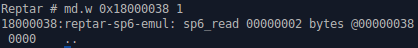
\includegraphics[width=12cm]{TestReadFPGA.png}
\end{center}
\vspace{1cm} 

\pagebreak

\subsection{Etape 3}
Dans cette étape nous avons créé l'émulation des LEDs de la FPGA. Nous nous sommes basés sur les codes existants dans le répertoire. Voici ci-dessous le code d'émulation des LEDs : 

\lstinputlisting[label=Qemu LEDs,caption=reptar\_sp6\_leds.h,language=C]{Ressources/Code_Source/reptar_sp6_leds.h}
\vspace{0.5cm} 
\lstinputlisting[label=Qemu LEDs,caption=reptar\_sp6\_leds.c,language=C]{Ressources/Code_Source/reptar_sp6_leds.c}
\vspace{0.5cm} 

L'émulation est extrêmement simple. Cela consiste en trois fonctions : "init", "read" et "write". Nous avons utilisé les registres 16 bits fournis dans notre structure "opaque" pour stocker l'états des 8 LEDs.

La fonction "write" crée un commande JSON qui est envoyé par un socket vers l'interface Qt.

Pour tester le fonctionnement des LEDs, nous avons utilisé, comme proposé dans la donnée du laboratoire, la commande "itbok" de U-Boot, avec le test numéro 10. Voici le résultat :

\begin{center} 
\hspace{12.45cm}
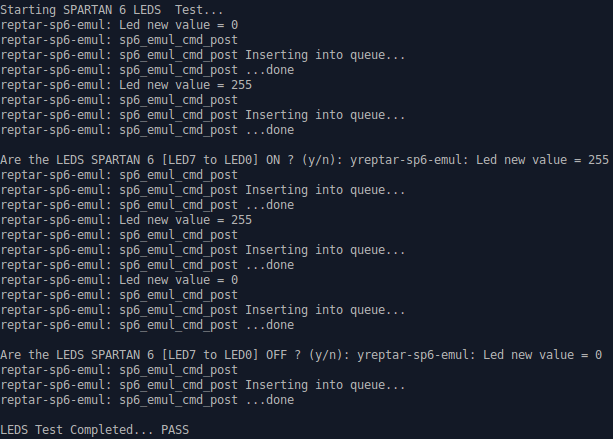
\includegraphics[width=16cm]{TestLEDs.png}
\end{center}
\vspace{1cm} 

\pagebreak

\subsection{Etape 4}
Dans cette étape nous avons émulé les boutons poussoirs de la FPGA. 

Voici ci-dessous le code d'émulation des boutons : 

\lstinputlisting[label=Qemu LEDs,caption=reptar\_sp6\_buttons.h,language=C]{Ressources/Code_Source/reptar_sp6_buttons.h}
\vspace{0.5cm} 
\lstinputlisting[label=Qemu LEDs,caption=reptar\_sp6\_buttons.c,language=C]{Ressources/Code_Source/reptar_sp6_buttons.c}
\vspace{0.5cm} 

Ce module est encore plus simple que les LEDs. Ici on n'a pas besoin de gérer l'écriture (on ne peut pas assigner une valeur à des boutons). La seule différence est que cette fois, on recois des évenenements JSON de l'interface Qt lorsqu'un bouton à été pressé.\\

Nous avons aussi utilisé les registres de la structure "opaque" pour stocker les valeurs des boutons. Comme on peut aussi le constater, a chaque évennement de pression sur un bouton, nous appellons la fonction d'IRQ pour les boutons (voir étape suivante).

Pour tester les boutons nous avons utilisé l'application fournie "sp6\_buttons\_u-boot". Voici le résultat.

\begin{center} 
\hspace{12.45cm}
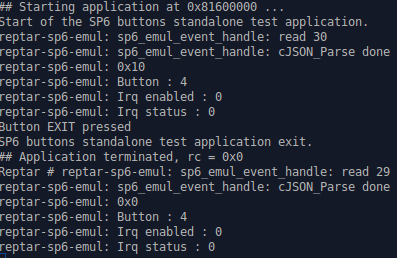
\includegraphics[width=12cm]{TestButtons.png}
\end{center}
\vspace{1cm} 

\pagebreak
\subsection{Etape 5}
Cette étape nous à permis de mettre en place le système d'interruption. 
Voici ci-dessous le code développé à cet effet : 

\lstinputlisting[label=Qemu LEDs,caption=reptar\_sp6\_irq.h,language=C]{Ressources/Code_Source/reptar_sp6_irq.h}
\vspace{0.5cm} 
\lstinputlisting[label=Qemu LEDs,caption=reptar\_sp6\_irq.c,language=C]{Ressources/Code_Source/reptar_sp6_irq.c}
\vspace{0.5cm} 

Pour cette partie, nous avons utilisé la puissance des champs de bits du C. Il y a pour l'instant quatre fonctions principales : "read", "write", "init" et "irq\_button". Les fonction de lecture et écriture respective permettent d'accéder aux registres IRQ de la FPGA. La fonction "reptar\_sp6\_irq\_button" permet de générer une interruption à chaque événement des boutons.  \\


Pour tester cette IRQ avec u-boot, voici comment nous avons procédé :
\begin{lstlisting}[language=C,caption=Commandes u-boot]
mw.l 0x4831001C 0x00000400 1	//set bit 10 of GPIO_IRQENABLE1 to 1
mw.l 0x48310048 0x00000400 1	//set bit 10 of GPIO_RISINGDETECT to 1
mw.w 0x18000018 0x0080 1	//enable the IRQ in FPGA

md.l 0x48310018 1		//displays GPIO_IRQSTATUS1 register (bit 10 should be 0)
md.w 0x18000018 1		//displays the IRQ_CTL_REG of FPGA  (should be 0x0080)

//press the button 4

md.l 0x48310018 1		//displays GPIO_IRQSTATUS1 register (bit 10 should be 1)
md.w 0x18000018 1		//displays the IRQ_CTL_REG of FPGA  (should be 0x0098)
\end{lstlisting}



Et voici le résultat obtenu (adresse 0x18000018 valant bien 0x0098 et adresse 0x48310018 avec le bit 10 à 1, comme attendu) :
\begin{center} 
\hspace{12.45cm}
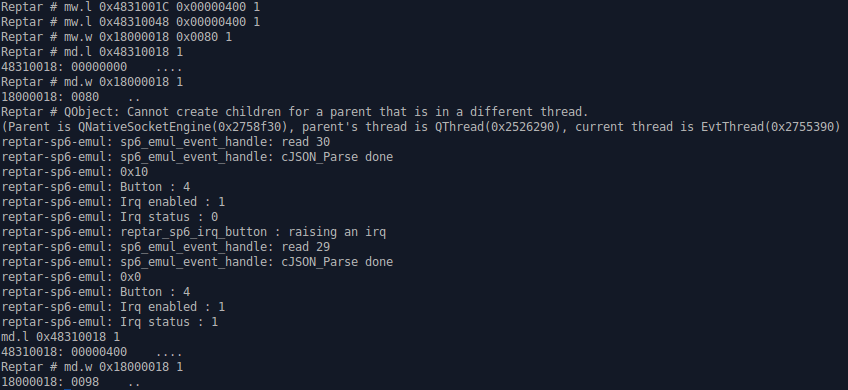
\includegraphics[width=16cm]{TestIRQ.png}
\end{center}
\vspace{1cm} 


\pagebreak
\subsection{Etape 6}
Dans cette étape nous avons émulé l'affichage 7 segments :
\lstinputlisting[label=Qemu LEDs,caption=reptar\_sp6\_7segs.h,language=C]{Ressources/Code_Source/reptar_sp6_7segs.h}
\vspace{0.5cm} 
\lstinputlisting[label=Qemu LEDs,caption=reptar\_sp6\_7segs.c,language=C]{Ressources/Code_Source/reptar_sp6_7segs.c}
\vspace{0.5cm} 

La complexité de ce module est exactement identique à celui des LEDs (sauf qu'il faut juste gérer 3 registres identique). Nous avons, comme dans les autres modules, utilisé les registres de la structure "opaque" pour stocker l'état des registres. Le JSON nous permet de mettre à jour le programme "Qt", exactement comme pour les LEDs.\\

\textit{\textbf{Remarques} : L'API proposée dans le document n'est pas très claire quant aux valeurs à envoyer. On ne peut pas gérer les segments séparément (ce qui serait logique), mais on ne peut les allumer que si cela correspond à un chiffre de 0 à 9 ! }\\


Pour tester ce code nous avons utilisé l'application fournie "7seg\_u-boot". Voici le résultat :

\begin{center} 
\hspace{12.45cm}
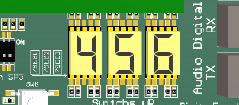
\includegraphics[width=8cm]{Test7Segs.png}
\end{center}
\vspace{1cm} 

\pagebreak
\subsection{Etape 7}
Dans cette étape nous avons fait une application fonctionnant dans u-boot qui utilise les boutons ainsi que les afficheurs 7 segments.

Cette application contient une fonction "main" ainsi qu'une fonction pour afficher les 7 segments et une autre pour lire les boutons :

\begin{lstlisting}[language=C,caption=main]
#include <common.h>
#include <command.h>
#include <asm/arch/mux.h>
#include <asm/io.h>
#include <asm/errno.h>
#include "board/ti/reptar/reptar.h"

#define SW2 0x02
#define SW3 0x04
#define SW4 0x08
#define SW5 0x80

#define N_DELAY 0x2E8

extern int sevenseg_putc(int index, unsigned char number);
extern int buttons_read(void);

int main(int argc, char *argv[]) {
	printf("Start of the Miniapp U-boot Standalone Application\n");

	char end = 0;
	char buttons = 0;
	char buttonsOld = 0;
	char dig1 = 0, dig2 = 0, dig3 = 0;
	int j;

	sevenseg_putc(0, 0);
	sevenseg_putc(1, 0);
	sevenseg_putc(2, 0);

	while (!end) {

		//anti rebonds
		j = N_DELAY;
		while (j--)
			;

		//lire les boutons
		buttons = buttons_read();

		//vérifier les états des boutons
		if (!(buttonsOld & SW2) && (buttons & SW2)) {
			dig1++;
			if (dig1 == 10)
				dig1 = 0;
			sevenseg_putc(0, dig1);
		}

		if (!(buttonsOld & SW5) && (buttons & SW5)) {
			dig2++;
			if (dig2 == 10)
				dig2 = 0;
			sevenseg_putc(1, dig2);
		}

		if (!(buttonsOld & SW4) && (buttons & SW4)) {
			dig3++;
			if (dig3 == 10)
				dig3 = 0;
			sevenseg_putc(2, dig3);
		}

		if (!(buttonsOld & SW3) && (buttons & SW3))
			end = 1;

		buttonsOld = buttons;
	}

	printf("Stop of the Miniapp U-boot Standalone Application\n");

	return 0;
}
\end{lstlisting}

\begin{lstlisting}[language=C,caption=7segs]
/**
* A character is encoded on 8 bits
*
* BIT0: Encode segment "a"
* BIT1: Encode segment "b"
* BIT2: Encode segment "c"
* BIT3: Encode segment "d"
* BIT4: Encode segment "e"
* BIT5: Encode segment "f"
* BIT6: Encode segment "g"
* BIT7: Encode segment "dot point"
*
* 0: fedcba => 00111111 => 0x3F
* 1: cb     => 00000110 => 0x06
* 2: gedba  => abged => 0x5B
* 3: abgcd  => 01001111 => 0x4F
* 4: fgbc   => 01100110 => 0x66
* 5: afgcd  => 01101101 => 0x6D
* 6: afgecd => 01111101 => 0x7D
* 7: abc    => 00000111 => 0x07
* 8: abcdefg=> 01111111 => 0x7F
* 9: afgbcd => 01101111 => 0x6F
*
*/

#include <asm/io.h>
#include <common.h>
#include <errno.h>
#include "board/ti/reptar/reptar.h"

#define N_CHARS 10

static u32 register_addr[] = {
	SP6_DISP_7SEG1,
	SP6_DISP_7SEG2,
	SP6_DISP_7SEG3,
};

const u16 char2seg[N_CHARS] = {
	0x3F, 0x06, 0x5B, 0x4F, 0x66, 0x6D, 0x7D, 0x07, 0x7F, 0x6F
};

int sevenseg_putc(int index, unsigned char number)
{
	u16 c;

	if ((index < 0) || (index > 2))
		return -EINVAL;

	if ((number < 0) || (number > N_CHARS))
		return -EINVAL;

	c = char2seg[(int)number];
	writew(c, register_addr[index]);

	return 0;
}
\end{lstlisting}

\begin{lstlisting}[language=C,caption=boutons]
/*
 * buttons.c
 *
 *  Created on: Apr 19, 2016
 *      Author: redsuser
 */

#include <asm/io.h>
#include <common.h>
#include <errno.h>
#include "board/ti/reptar/reptar.h"

int buttons_read(void)
{
	u16 regval;

	regval = readw(SP6_PUSH_BUT);

	return (regval & 0x00FF);
}
\end{lstlisting}

Lors d’un appui sur SW2, SW5 ou SW4, le digit respectivement à gauche, au centre ou au milieu est incrémenté de 1, modulo 10 : Si un digit atteint 9, il revient à 0. Au démarrage, l'application affiche "000" sur les 7 segments. Un appui sur SW3 quitte l'application.\\

Pour tester ce code nous avons lancé l'application dans u-boot et pressé les boutons. Voici le résultat :

\begin{center} 
\hspace{12.45cm}
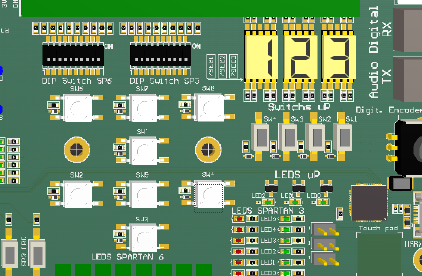
\includegraphics[width=8cm]{Miniapp.png}
\end{center}
\vspace{1cm} 